\section{Continual Graph Learning with EWC}
\label{sec:continual}

\subsection{Typology Concept Drift & Catastrophic Forgetting}
In operational AML deployment, financial crime networks adapt their behavioral patterns over time. When a supervised neural model is updated on novel typologies (Task B), gradient descent updates parameters along directions that minimize loss on Task B, inadvertently destroying the parameter configurations necessary to identify base typologies (Task A).

\begin{figure}[t]
\centering
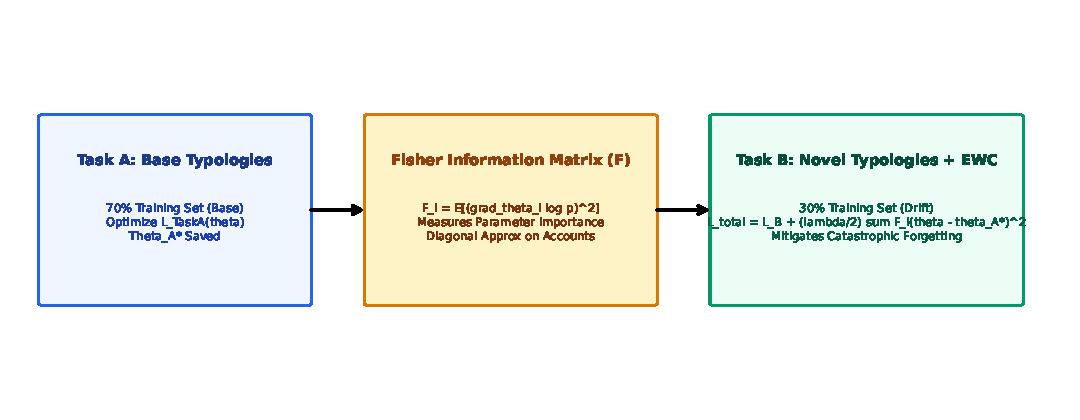
\includegraphics[width=\columnwidth]{figures/fig4_workflow.pdf}
\caption{Workflow of the Continual Graph Learning framework with Elastic Weight Consolidation (EWC), illustrating Fisher Information Matrix extraction on Task A and quadratic regularization on Task B.}
\label{fig:ewc_workflow}
\end{figure}

\subsection{Elastic Weight Consolidation (EWC) Formulation}
To mitigate catastrophic forgetting while maintaining plasticity, we adapt Elastic Weight Consolidation~\cite{kirkpatrick2017overcoming} to the AMECF architecture. Following convergence on Task A with optimal parameter configuration $\theta_A^*$, the empirical Fisher Information Matrix $\mathbf{F}$ is computed across the training accounts:
\begin{equation}
    F_i = \mathbb{E}_{u \in \mathcal{V}_{\text{train}}^A} \left[ \left( \frac{\partial \log P(y_u \mid \mathcal{G}_{\text{safe}}; \theta)}{\partial \theta_i} \right)^2 \right]_{\theta = \theta_A^*}
    \label{eq:fisher}
\end{equation}
where $F_i$ represents the diagonal element of the Fisher Information Matrix corresponding to parameter $\theta_i$, quantifying how sensitive the Task A predictive distribution is to perturbations in $\theta_i$.

When training on Task B, the loss function is augmented with a quadratic EWC penalty:
\begin{equation}
    \mathcal{L}_{\text{total}}(\theta) = \mathcal{L}_{\text{Task B}}(\theta) + \sum_{i} \frac{\lambda}{2} F_i (\theta_i - \theta_{A, i}^*)^2
    \label{eq:ewc_loss}
\end{equation}
where $\lambda \ge 0$ is a scalar hyperparameter governing the stability-plasticity tradeoff.

\subsection{Continual Optimization Procedure}
The complete continual optimization procedure operates in three sequential stages:
\begin{enumerate}
    \item \textbf{Base Task Optimization:} The AMECF parameters $\theta$ are trained on Task A accounts $\mathcal{V}_{\text{train}}^A$ via class-weighted cross-entropy until convergence, yielding optimal base parameters $\theta_A^*$.
    \item \textbf{Diagonal Fisher Computation:} The diagonal Fisher information tensor $\{F_i\}$ is calculated across sampled Task A accounts via Eq.~\eqref{eq:fisher}.
    \item \textbf{Task B Adaptation with Quadratic Penalty:} During Task B optimization over $\mathcal{V}_{\text{train}}^B$, gradients are computed jointly over the task cross-entropy and the Fisher-weighted quadratic distance to $\theta_A^*$ (Eq.~\eqref{eq:ewc_loss}).
\end{enumerate}
